% Created by tikzDevice version 0.12.6 on 2026-08-03 04:28:35
% !TEX encoding = UTF-8 Unicode
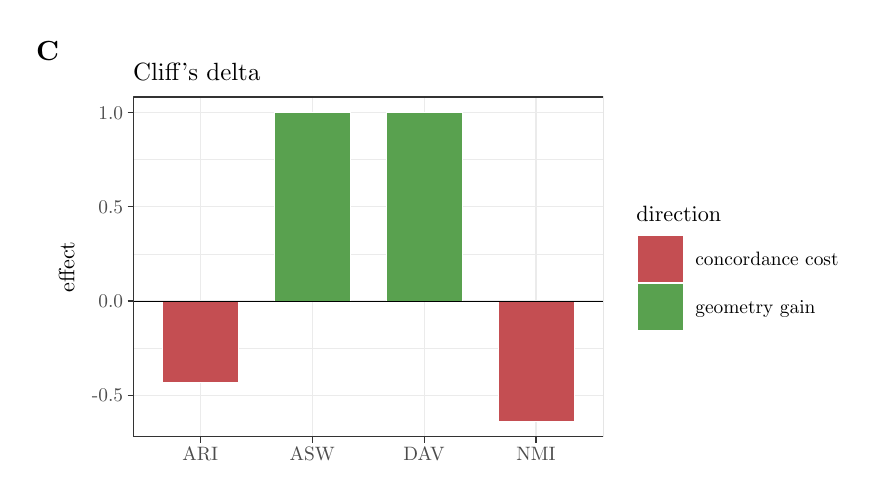
\begin{tikzpicture}[x=1pt,y=1pt]
\definecolor{fillColor}{RGB}{255,255,255}
\path[use as bounding box,fill=fillColor,fill opacity=0.00] (0,0) rectangle (303.38,161.83);
\begin{scope}
\path[clip] (  1.05,  1.74) rectangle (302.34,160.09);
\definecolor{drawColor}{RGB}{255,255,255}
\definecolor{fillColor}{RGB}{255,255,255}

\path[draw=drawColor,line width= 0.4pt,line join=round,line cap=round,fill=fillColor] (  1.05,  1.74) rectangle (302.34,160.09);
\end{scope}
\begin{scope}
\path[clip] ( 38.09, 13.93) rectangle (207.93,136.79);
\definecolor{fillColor}{RGB}{255,255,255}

\path[fill=fillColor] ( 38.09, 13.93) rectangle (207.93,136.79);
\definecolor{drawColor}{gray}{0.92}

\path[draw=drawColor,line width= 0.2pt,line join=round] ( 38.09, 46.03) --
	(207.93, 46.03);

\path[draw=drawColor,line width= 0.2pt,line join=round] ( 38.09, 80.10) --
	(207.93, 80.10);

\path[draw=drawColor,line width= 0.2pt,line join=round] ( 38.09,114.17) --
	(207.93,114.17);

\path[draw=drawColor,line width= 0.4pt,line join=round] ( 38.09, 28.99) --
	(207.93, 28.99);

\path[draw=drawColor,line width= 0.4pt,line join=round] ( 38.09, 63.06) --
	(207.93, 63.06);

\path[draw=drawColor,line width= 0.4pt,line join=round] ( 38.09, 97.13) --
	(207.93, 97.13);

\path[draw=drawColor,line width= 0.4pt,line join=round] ( 38.09,131.21) --
	(207.93,131.21);

\path[draw=drawColor,line width= 0.4pt,line join=round] ( 62.36, 13.93) --
	( 62.36,136.79);

\path[draw=drawColor,line width= 0.4pt,line join=round] (102.79, 13.93) --
	(102.79,136.79);

\path[draw=drawColor,line width= 0.4pt,line join=round] (143.23, 13.93) --
	(143.23,136.79);

\path[draw=drawColor,line width= 0.4pt,line join=round] (183.67, 13.93) --
	(183.67,136.79);
\definecolor{drawColor}{RGB}{255,255,255}
\definecolor{fillColor}{RGB}{196,78,82}

\path[draw=drawColor,line width= 0.2pt,fill=fillColor] (169.92, 19.52) rectangle (197.42, 63.06);

\path[draw=drawColor,line width= 0.2pt,fill=fillColor] ( 48.61, 33.69) rectangle ( 76.11, 63.06);
\definecolor{fillColor}{RGB}{89,161,79}

\path[draw=drawColor,line width= 0.2pt,fill=fillColor] ( 89.05, 63.06) rectangle (116.54,131.21);

\path[draw=drawColor,line width= 0.2pt,fill=fillColor] (129.48, 63.06) rectangle (156.98,131.21);
\definecolor{drawColor}{RGB}{0,0,0}

\path[draw=drawColor,line width= 0.3pt,line join=round] ( 38.09, 63.06) -- (207.93, 63.06);
\definecolor{drawColor}{gray}{0.20}

\path[draw=drawColor,line width= 0.4pt,line join=round,line cap=round] ( 38.09, 13.93) rectangle (207.93,136.79);
\end{scope}
\begin{scope}
\path[clip] (  0.00,  0.00) rectangle (303.38,161.83);
\definecolor{drawColor}{gray}{0.30}

\node[text=drawColor,anchor=base east,inner sep=0pt, outer sep=0pt, scale=  0.70] at ( 34.49, 26.58) {-0.5};

\node[text=drawColor,anchor=base east,inner sep=0pt, outer sep=0pt, scale=  0.70] at ( 34.49, 60.65) {0.0};

\node[text=drawColor,anchor=base east,inner sep=0pt, outer sep=0pt, scale=  0.70] at ( 34.49, 94.72) {0.5};

\node[text=drawColor,anchor=base east,inner sep=0pt, outer sep=0pt, scale=  0.70] at ( 34.49,128.80) {1.0};
\end{scope}
\begin{scope}
\path[clip] (  0.00,  0.00) rectangle (303.38,161.83);
\definecolor{drawColor}{gray}{0.20}

\path[draw=drawColor,line width= 0.4pt,line join=round] ( 36.09, 28.99) --
	( 38.09, 28.99);

\path[draw=drawColor,line width= 0.4pt,line join=round] ( 36.09, 63.06) --
	( 38.09, 63.06);

\path[draw=drawColor,line width= 0.4pt,line join=round] ( 36.09, 97.13) --
	( 38.09, 97.13);

\path[draw=drawColor,line width= 0.4pt,line join=round] ( 36.09,131.21) --
	( 38.09,131.21);
\end{scope}
\begin{scope}
\path[clip] (  0.00,  0.00) rectangle (303.38,161.83);
\definecolor{drawColor}{gray}{0.20}

\path[draw=drawColor,line width= 0.4pt,line join=round] ( 62.36, 11.93) --
	( 62.36, 13.93);

\path[draw=drawColor,line width= 0.4pt,line join=round] (102.79, 11.93) --
	(102.79, 13.93);

\path[draw=drawColor,line width= 0.4pt,line join=round] (143.23, 11.93) --
	(143.23, 13.93);

\path[draw=drawColor,line width= 0.4pt,line join=round] (183.67, 11.93) --
	(183.67, 13.93);
\end{scope}
\begin{scope}
\path[clip] (  0.00,  0.00) rectangle (303.38,161.83);
\definecolor{drawColor}{gray}{0.30}

\node[text=drawColor,anchor=base,inner sep=0pt, outer sep=0pt, scale=  0.70] at ( 62.36,  5.51) {ARI};

\node[text=drawColor,anchor=base,inner sep=0pt, outer sep=0pt, scale=  0.70] at (102.79,  5.51) {ASW};

\node[text=drawColor,anchor=base,inner sep=0pt, outer sep=0pt, scale=  0.70] at (143.23,  5.51) {DAV};

\node[text=drawColor,anchor=base,inner sep=0pt, outer sep=0pt, scale=  0.70] at (183.67,  5.51) {NMI};
\end{scope}
\begin{scope}
\path[clip] (  0.00,  0.00) rectangle (303.38,161.83);
\definecolor{drawColor}{RGB}{0,0,0}

\node[text=drawColor,rotate= 90.00,anchor=base,inner sep=0pt, outer sep=0pt, scale=  0.80] at ( 16.86, 75.36) {effect};
\end{scope}
\begin{scope}
\path[clip] (  0.00,  0.00) rectangle (303.38,161.83);
\definecolor{fillColor}{RGB}{255,255,255}

\path[fill=fillColor] (215.93, 48.25) rectangle (300.34,102.47);
\end{scope}
\begin{scope}
\path[clip] (  0.00,  0.00) rectangle (303.38,161.83);
\definecolor{drawColor}{RGB}{0,0,0}

\node[text=drawColor,anchor=base west,inner sep=0pt, outer sep=0pt, scale=  0.80] at (219.93, 91.95) {direction};
\end{scope}
\begin{scope}
\path[clip] (  0.00,  0.00) rectangle (303.38,161.83);
\definecolor{fillColor}{RGB}{255,255,255}

\path[fill=fillColor] (219.93, 69.60) rectangle (237.27, 86.94);
\definecolor{drawColor}{RGB}{255,255,255}
\definecolor{fillColor}{RGB}{196,78,82}

\path[draw=drawColor,line width= 0.2pt,fill=fillColor] (220.21, 69.88) rectangle (236.99, 86.66);
\end{scope}
\begin{scope}
\path[clip] (  0.00,  0.00) rectangle (303.38,161.83);
\definecolor{fillColor}{RGB}{255,255,255}

\path[fill=fillColor] (219.93, 52.25) rectangle (237.27, 69.60);
\definecolor{drawColor}{RGB}{255,255,255}
\definecolor{fillColor}{RGB}{89,161,79}

\path[draw=drawColor,line width= 0.2pt,fill=fillColor] (220.21, 52.54) rectangle (236.99, 69.31);
\end{scope}
\begin{scope}
\path[clip] (  0.00,  0.00) rectangle (303.38,161.83);
\definecolor{drawColor}{RGB}{0,0,0}

\node[text=drawColor,anchor=base west,inner sep=0pt, outer sep=0pt, scale=  0.70] at (241.27, 75.86) {concordance cost};
\end{scope}
\begin{scope}
\path[clip] (  0.00,  0.00) rectangle (303.38,161.83);
\definecolor{drawColor}{RGB}{0,0,0}

\node[text=drawColor,anchor=base west,inner sep=0pt, outer sep=0pt, scale=  0.70] at (241.27, 58.51) {geometry gain};
\end{scope}
\begin{scope}
\path[clip] (  0.00,  0.00) rectangle (303.38,161.83);
\definecolor{drawColor}{RGB}{0,0,0}

\node[text=drawColor,anchor=base west,inner sep=0pt, outer sep=0pt, scale=  0.90] at ( 38.09,142.78) {Cliff's delta};
\end{scope}
\begin{scope}
\path[clip] (  0.00,  0.00) rectangle (303.38,161.83);
\definecolor{drawColor}{RGB}{0,0,0}

\node[text=drawColor,anchor=base,inner sep=0pt, outer sep=0pt, scale=  1.00] at (  7.20,150.08) {\bfseries C};
\end{scope}
\end{tikzpicture}
